
\documentclass{report}

\usepackage[utf8]{inputenc}
\usepackage[italian]{babel}
\usepackage{import}
\usepackage{todonotes}
\usepackage{color}
\usepackage{rotating}
\usepackage[hidelinks]{hyperref}
\usepackage{url}
\usepackage{pdfpages}
\usepackage{siunitx}
\usepackage{pdflscape}
\usepackage{subfig}
\usepackage[euler]{textgreek}
\usepackage{mhchem}

\usepackage{multirow}

\usepackage{enumerate} 
\usepackage{amsmath}
\usepackage{amsfonts}

\usepackage[signatures,swapnames,sans]{frontespizio}

\usepackage{geometry}
\geometry{portrait, margin=3cm}
\usepackage{siunitx}
\usepackage{booktabs}

\renewcommand*\figurename{Figura}

\newcommand{\sub}[1]{\textsubscript{#1}}
\newcommand{\super}[1]{\textsuperscript{#1}}
\newcommand{\parallelsum}{\mathbin{\!/\mkern-5mu/\!}}

\newcommand{\Fig}[0]{Fig.}

\usepackage{listings} %Per inserire codice
%\usepackage[usenames]{color} %Per permettere la colorazione dei caratteri

\lstnewenvironment{codice_arduino}[1][]
{\lstset{basicstyle=\small\ttfamily, columns=fullflexible,
keywordstyle=\color{red}\bfseries, commentstyle=\color{blue},
language=C++, basicstyle=\small,
numbers=left, numberstyle=\tiny,
stepnumber=2, numbersep=5pt, float=*, #1}}{}

\usepackage{titlesec}

\titleformat{\chapter}{\normalfont\huge}{}{20pt}{\huge\bfseries}

\linespread{1.3}


%% COMANDI UTILI
%\begin{table}[h]
%	\centering
%	\begin{tabular}{|c|c|c|}
%	\cline{2-3} 
%	\multicolumn{1}{c|}{} & \textbf{Valore nominale} & \textbf{Valore misurato}\\ 
%		%\hline
%		%{} & \textbf{Valore nominale} & \textbf{Valore misurato} \\ 
%		\hline
%		$\mathbf{R_1}$ & \SI{18}{k\ohm} & \SI{17.977}{k\ohm} \\ 
%		\hline
%		$\mathbf{R_2}$& \SI{1.8}{k\ohm} & \SI{1.815}{k\ohm} \\ 
%		\hline
%	\end{tabular}
%\caption{Misure delle resistenze utilizzate per il circuito.}
%\label{table:mis_res}
%\end{table}
%\begin{figure}[h!]
%\centering
%\includegraphics[height=6.5cm]{immagini/TEK00018}\\(a)\\[1ex]
%\includegraphics[height=6.5cm]{immagini/TEK00019}\\(b)
%\caption{Risposta del circuito con accoppiamento DC (a) e accoppiamento AC (b).}
%	\label{figura:accopp}
%\end{figure}

\begin{document}
%\addtocounter{chapter}{+4}
	\begin{frontespizio}
		\Margini{3cm}{3cm}{3cm}{3cm}
		\Universita{Bergamo}
		\Logo[43.332mm]{unibg-mark}
		\Divisione{Scuola di Ingegneria}
		\Corso[Laurea Magistrale]{Ingegneria Informatica}
		\Titolo{Laboratorio di Robotica}
		\Sottotitolo{Documentazione attività di laboratorio }
		\Punteggiatura{}
		\NRelatore{Prof.}{Prof.}
		\Relatore{Davide Brugali}
		\Candidato[1058231]{Giulia Allievi}
		\Candidato[1059640]{Martina Fanton}
		\Annoaccademico{2022--2023}
		\begin{Preambolo*}
			\usepackage[italian]{babel}
			\usepackage[T1]{fontenc}
			\usepackage[utf8]{inputenc}
			\usepackage{microtype}
			\usepackage{lmodern}
			\graphicspath{{img/}}
			
			\renewcommand{\frontinstitutionfont}{\fontsize{14}{17}\bfseries\scshape}
			\renewcommand{\fronttitlefont}{\fontsize{17}{21}\bfseries\scshape}
			\renewcommand{\frontfootfont}{\fontsize{12}{14}\bfseries\scshape}
		\end{Preambolo*}
	\end{frontespizio}

%----------------------------------------------------------------------------------------
%	PAGINA BIANCA
%----------------------------------------------------------------------------------------
%\newpage
%\null
%\thispagestyle{empty}
%\newpage

%----------------------------------------------------------------------------------------
%	INDICE
%----------------------------------------------------------------------------------------
\tableofcontents

%----------------------------------------------------------------------------------------
%	INTRO
%----------------------------------------------------------------------------------------
\chapter{Introduzione}
L'obiettivo del nostro progetto è quello di fornire le coordinate e l'orientamento della pinza ad un robot, al fine di potersi posizionare per afferrare un oggetto. Le coordinate e l'orientamento vengono calcolate da un'opportuna libreria (nel nostro caso dalla libreria \textit{Grasp Pose Generator, GPG}), la quale necessita delle informazioni dell'oggetto inquadrato sotto forma di una nuvola di punti, la point cloud, che verrà fornita attraverso la \textit{Stereo Camera ZED}. Il software del progetto sarà realizzato utilizzando il \textit{Framework STAR}. \par
La \textit{Stereo Camera ZED} è dotata di vari sensori, per esempio l'accelereometro e il giroscopio, ma nella nostra applicazione serviranno solo i dati delle immagini, in particolare solo quelli della point cloud. La fotocamera stereoscopica ha un range di profondità compreso fra \SI{30}{c\meter} e \SI{20}{\meter} (fonte: \textcolor{blue}{\underline{\href{https://www.stereolabs.com/assets/datasheets/zed2-camera-datasheet.pdf}{datasheet}}}), perciò gli oggetti da inquadrare dovranno essere posizionati ad una distanza compresa in questo intervallo. \par
Di seguito, nel capitolo \ref{librerie} verranno analizzate due diverse librerie che si possono utilizzare per ottenere i dati relativi alla posizione e all'orientamento della pinza del robot, mentre nel capitolo \ref{integrazione} verranno descritti i passi necessari per integrare, compilare ed eseguire il progetto. Infine, nel capitolo \ref{risultati} verranno mostrati i risultati finali.
\newpage
\chapter{Librerie}\label{librerie}
Prima di costruire l'applicazione finale (in cui è stata integrata soltanto la libreria GPG), sono state analizzate due diverse librerie \textit{stand-alone}, la \textit{Grasp Pose Generator} (GPG), la cui documentazione è reperibile al seguente link: \textcolor{blue}{\underline{\url{https://github.com/atenpas/gpg}}}, e la \textit{Grasp Pose Detection} (GPD), la cui documentazione è invece disponibile al seguente link: \textcolor{blue}{\underline{\url{https://github.com/atenpas/gpd}}}.\par
\section{Grasp Pose Generator (GPG)}\label{GPG}
Questa libreria permette di individuare, data la point cloud di un oggetto contenuta in un file di tipo \texttt{.pcd}, un certo numero di possibili pinze con cui il robot può afferrare l'oggetto stesso. Questo numero di pinze restituite in output viene definito dall'utente nel file di configurazione della libreria. I parametri contenuti nel file di configurazione sono descritti più in dettaglio nella sezione \ref{fileConfig}. \par
Per poter eseguire la libreria, innanzitutto si deve scaricare lo zip della libreria da Github (\textcolor{blue}{\underline{\href{https://github.com/atenpas/gpg}{link}}}) estraendone il contenuto, rinominandolo come \texttt{grasp\_candidates\_generator} e spostandolo in una directory scelta dall'utente. Poi vanno scaricate tutte le librerie che la libreria GPG richiede per il suo funzionamento, ovvero \textit{PCL} (necessaria per elaborare la point cloud), \textit{Eigen} (necessaria per eseguire operazioni con vettori e matrici) e \textit{VTK} (necessaria per la visualizzazione della point cloud e delle prese), aprendo un nuovo terminale ed eseguendo in esso i comandi:
\begin{verbatim}
  sudo apt install libpcl-dev
  sudo apt install libeigen3-dev
  sudo apt-get install vtk6
\end{verbatim}
Ora si può procedere con l'esecuzione della libreria GPG. Per prima cosa si effettua la compilazione eseguendo nel precedente terminale i seguenti comandi:
\begin{verbatim}
  cd <location_of_your_workspace>  
  cd grasp_candidates_generator
  mkdir build && cd build
  cmake ..
  make
  sudo make install
\end{verbatim}
Successivamente va eseguito anche il prossimo comando per l'esecuzione effettiva della libreria:
\begin{verbatim}
  ./generate_candidates ../cfg/params.cfg ~/data/<point_cloud_name_file>.pcd
\end{verbatim}
In questo modo si visualizza a video un disegno in cui vengono visualizzati i vettori normali alla superficie inquadrata, per visualizzare la point cloud dell'oggetto in uno spazio tridimensionale con le pinze individuate dalla libreria è necessario cliccare il tasto Q sulla tastiera. Per chiudere anche questa nuova finestra va premuto nuovamente il tasto Q. Per entrambe le finestre, per cambiare lo zoom bisogna usare lo scroller del mouse, per muoversi sulla point cloud bisogna invece trascinare con il cursore. Nella figura \ref{figura:imggpg} sono riportate le due immagini. 
\begin{figure}[h!]
	\centering
	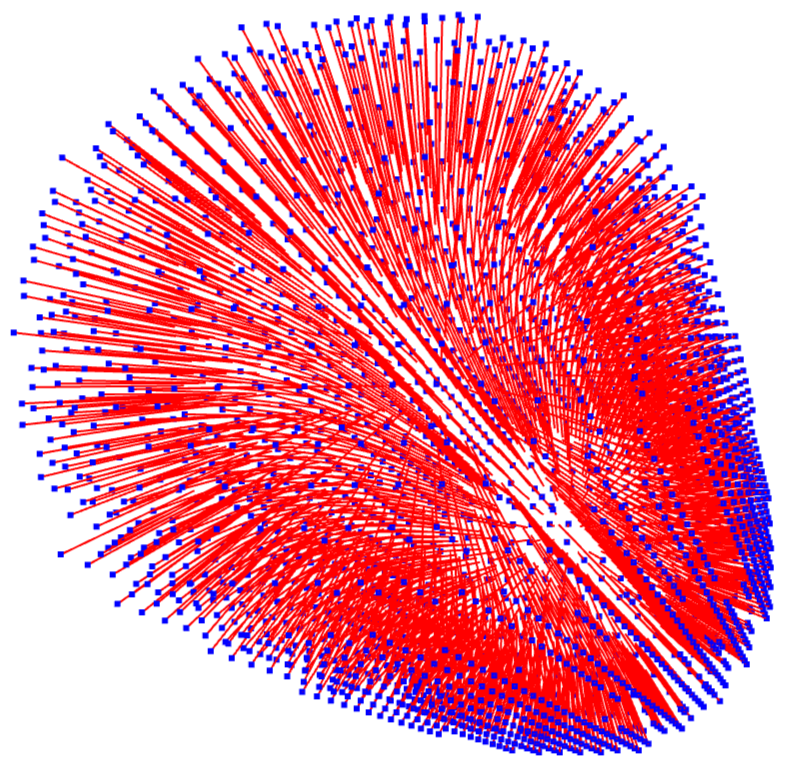
\includegraphics[height=5.5cm]{immagini/gpg1}
	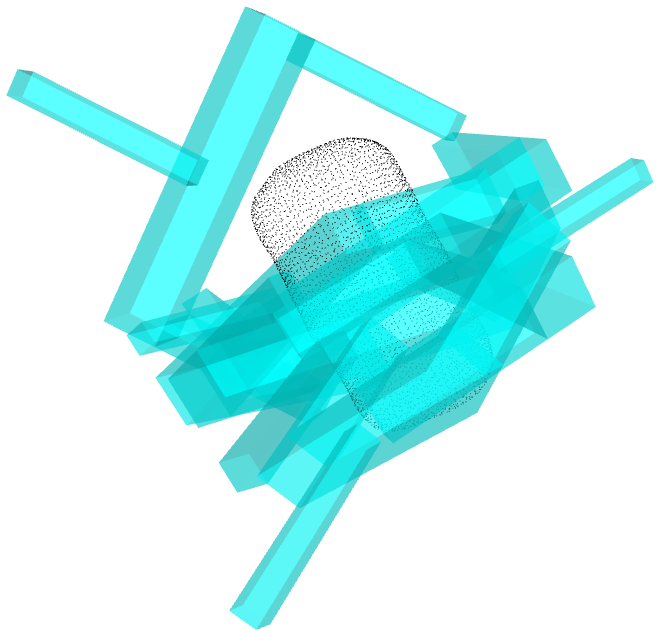
\includegraphics[height=5.5cm]{immagini/gpg2}
	\caption{Vettori normali alla superficie (a sinistra) e point cloud con sei possibili prese (a destra).}
	\label{figura:imggpg}
\end{figure}
\section{Grasp Pose Detection (GPD)}\label{GPD}
La libreria \textit{Grasp Pose Detection} è l'evoluzione della libreria \textit{Grasp Pose Generator} appena descritta. A differenza della libreria precedente, in questa libreria è integrato anche un classificatore per riconoscere gli oggetti afferrabili. La libreria GPD restituisce in output le pinze individuate, analogamente alla libreria GPG, ma per ogni presa viene specificato anche il suo score, che nell'immagine viene reso utilizzando dei diversi colori (verde per le pinze con score maggiore, che sono quelle corrette; giallo e arancione per quelle di score intermedio, che sono le prese accettabili; rosso per quelle con score basso, che sono da considerarsi non accettabili). Anche per questa libreria il numero delle pinze è definito dall'utente nel file di configurazione. \par
Per poter eseguire la libreria, innanzitutto si deve scaricare lo zip della libreria da Github (\textcolor{blue}{\underline{\href{https://github.com/atenpas/gpd}{link}}}) estraendone il contenuto, rinominandolo come \texttt{gpd} e spostandolo in una directory scelta dall'utente. Poi vanno scaricate tutte le librerie che la libreria GPD richiede per il suo funzionamento, ovvero \textit{PCL} (necessaria per elaborare la point cloud), \textit{Eigen} (necessaria per eseguire operazioni con vettori e matrici), \textit{VTK} (necessaria per la visualizzazione della point cloud e delle prese) e \textit{OpenCV} (necessaria per eseguire la detection delle pinze), aprendo un nuovo terminale ed eseguendo in esso i comandi:
\begin{verbatim}
  sudo apt install libpcl-dev
  sudo apt install libeigen3-dev
  sudo apt-get install vtk6
  sudo apt install libopencv-dev
\end{verbatim}
Ora si può procedere con l'esecuzione della libreria GPD. Per prima cosa si effettua la compilazione eseguendo nel precedente terminale i seguenti comandi:
\begin{verbatim}
  cd <location_of_your_workspace> 
  cd gpd
  mkdir build && cd build
  cmake ..
  make -j
  sudo make install
\end{verbatim}
Successivamente va eseguito anche il prossimo comando per l'esecuzione effettiva della libreria:
\begin{verbatim}
  ./detect_grasps ../cfg/eigen_params.cfg ../tutorials/krylon.pcd
\end{verbatim}
Questo comando viene eseguito sulla point cloud contenuta nel file \texttt{krylon.pcd} fornito da esempio dalla libreria, ma nel comando può essere inserito qualsiasi altro file di tipo \texttt{.pcd}. \par
In questo modo si visualizzano a video i vettori normali alla superficie della point cloud in uno spazio tridimensionale, però per visualizzare anche le pinze individuate dalla libreria è necessario cliccare nella tastiera sul tasto Q. Per vedere il numero scelto di pinze migliori, che  vengono distinte in base al loro colore secondo lo score che le caratterizza, è necessario premere di nuovo il tasto Q. Per chiudere anche questa nuova finestra va premuto nuovamente il tasto Q. Le immagini descritte sono riportate in figura \ref{figura:imggpd}, invece le informazioni sullo score mostrate a terminale si trovano in figura \ref{figura:imggpdt}.
\begin{figure}[h!]
	\centering
	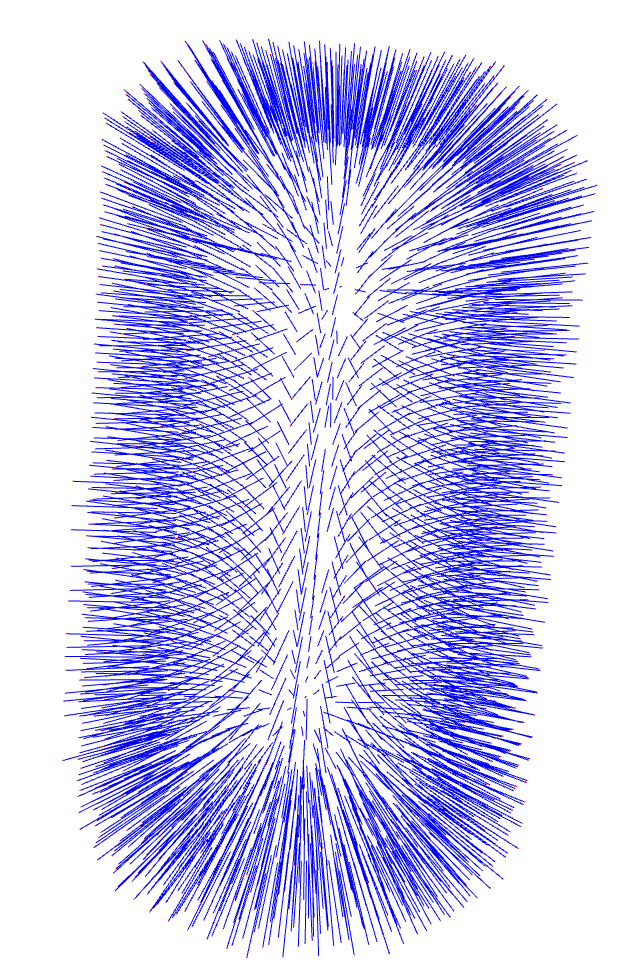
\includegraphics[height=5.4cm]{immagini/gpd1}
	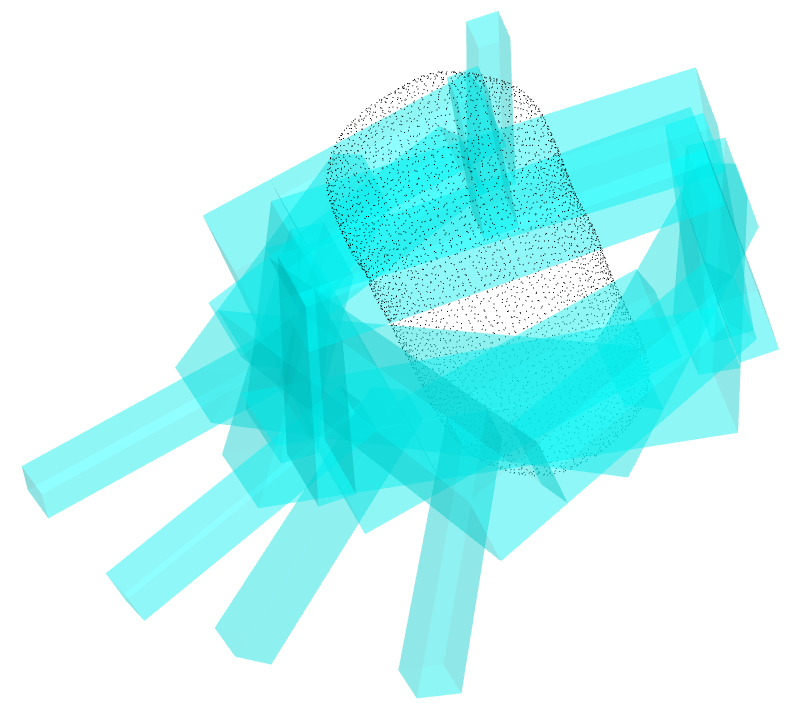
\includegraphics[height=5.4cm]{immagini/gpd2}
	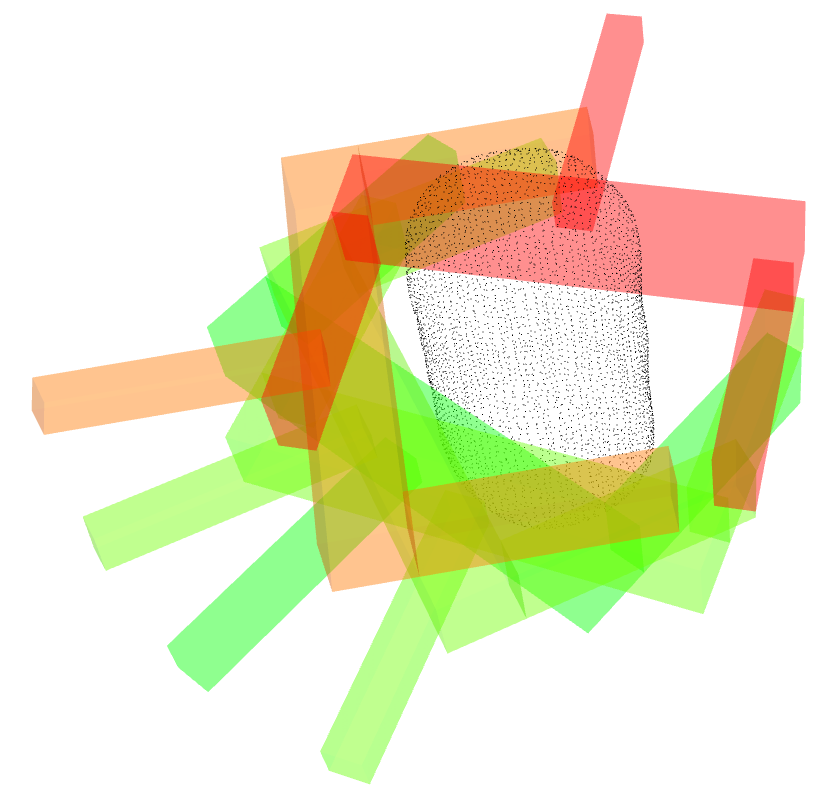
\includegraphics[height=5.4cm]{immagini/gpd3}
	\caption{Vettori normali alla superficie (a sinistra), point cloud con le possibili prese (al centro) e point cloud con le cinque migliori prese (a destra).}
	\label{figura:imggpd}
\end{figure}
\begin{figure}[h!]
	\centering
	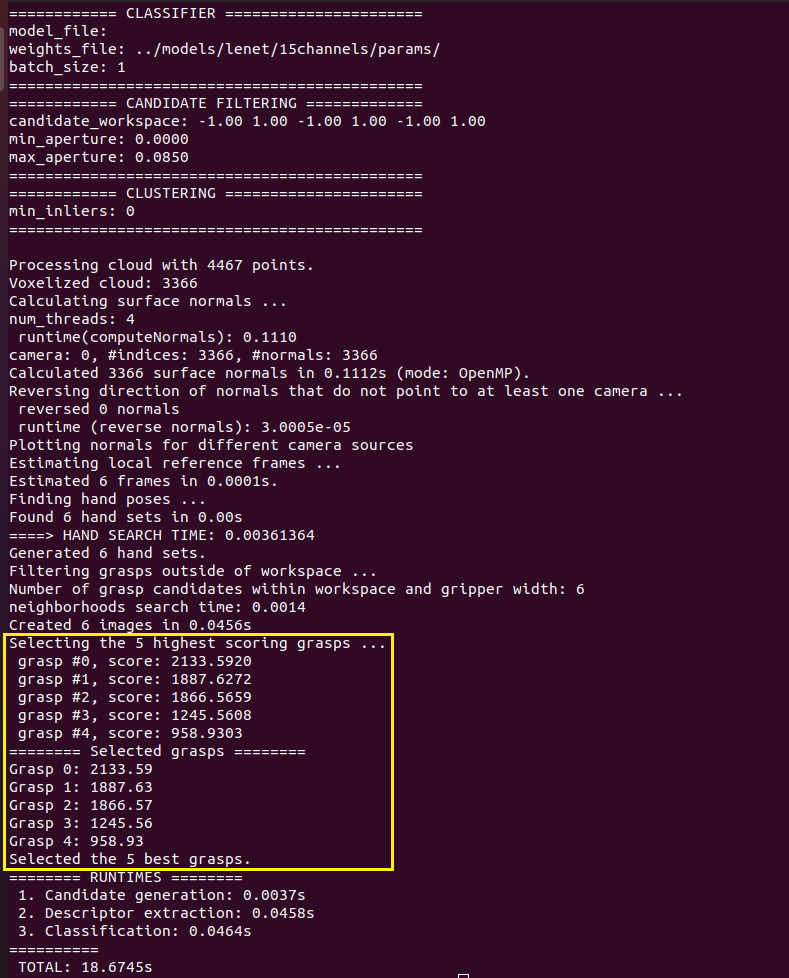
\includegraphics[width=\textwidth]{immagini/gpd4}
	\caption{Informazioni mostrate a terminale, quelle relative allo score si trovano nel riquadro evidenziato.}
	\label{figura:imggpdt}
\end{figure}
\newpage
\chapter{Integrazione}\label{integrazione}
In questo capitolo, verranno descritti i passi seguiti per ottenere l'applicazione finale. Innanzitutto è importante inizializzare le variabili d'ambiente di STAR in un nuovo terminale. Per fare ciò, bisogna eseguire questi comandi nel terminale:
\begin{verbatim}
  cd STAR
  cd AutonomousRobots
  . env-star.sh
\end{verbatim}
A questo punto, si inserisce la password (che è \texttt{unibg}) ed il terminale è pronto per essere utilizzato. L'inizializzazione va ripetuta ogni volta che si vuole utilizzare un nuovo terminale per eseguire delle azioni su STAR. 
\section{Libraries}
Per prima cosa, andiamo a copiare e compilare la libreria GPG descritta nella sezione precedente nella sottocartella \texttt{others} della cartella \texttt{Libraries} di STAR. Per fare ciò eseguiamo i seguenti comandi in un terminale, dopo aver raggiunto la cartella \texttt{others}:
\begin{verbatim}
  cd gpg
  mkdir build && cd build
  cmake ..
  make
  sudo make install
\end{verbatim}
Per eseguire la libreria, si deve digitare il comando seguente all'interno della cartella \texttt{build}:
\begin{verbatim}
  ./generate_candidates ../cfg/params.cfg 
  ~/STAR/AutonomousRobots/Libraries/others/gpg/tutorials/krylon.pcd
\end{verbatim}
La libreria appena importata funziona fornendogli in ingresso un file con estensione \texttt{.pcd} che contiene le informazioni sui punti della point cloud, però nel nostro caso la point cloud non sarà salvata su un file, ma verrà fornita dalla fotocamera stereoscopica. Modifichiamo quindi la libreria per fare in modo che riceva in ingresso non un file, ma una struttura dati denominata \texttt{CloudCamera} che è un riferimento alla struttura dati \texttt{pcl::PointCloud$<$pcl::PointXYZRGBA$>$::Ptr}. Quest'ultima variabile è un vettore contenente dei punti nel formato XYZRGBA: ogni punto è caratterizzato da 4 campi, i primi tre (X, Y, e Z) sono di tipo double e contengono le informazioni relative alle coordinate di quel punto in metri, invece l'ultimo campo, RGBA, è un intero senza segno a 32 bit in cui si codifica l'informazione sul colore. Ogni parametro del colore (R, G, B e A) è memorizzato in 8 bit e questo significa che ognuno di questi valori può variare da 0 a 255, perciò possono essere rappresentati fino a $\displaystyle{2^{32}=4.294.967.296}$ colori. Nello specifico, gli 8 bit meno significativi contengono l'informazione relativa al colore blu (B), i bit da 9 a 16 contengono l'informazione del colore verde (G), i bit da 17 a 24 codificano il valore del rosso (R), infine i bit da 25 a 32 contengono l'informazione del parametro alfa (A), che indica la trasparenza del colore. Nella nostra applicazione non utilizzeremo quest'informazione perché la point cloud è formata solo da punti di colore nero, che viene codificato dal valore più basso, ovvero 0. Per ottenere la modifica appena descritta, cambiamo il parametro della funzione \texttt{CandidatesGenerator::generateGraspCan-}\\\texttt{didates}, che non sarà più una stringa contenente il percorso del file, ma una varibalie di tipo \texttt{const CloudCamera\&}. \par
La seconda modifica che apportiamo riguarda il tipo restituito dalla funzione \texttt{CandidatesGenerator-}\\\texttt{::generateGraspCandidates}, perché non sarà più di tipo \texttt{std::vector<Grasp>} ma \texttt{void}. Il vettore delle prese viene aggiornato passando alla funzione l'indirizzo della variabile da aggiornare, perciò la funzione di partenza avrà un parametro aggiuntivo. \par 
A seguito di queste due modifiche, la segnatura della funzione \texttt{CandidatesGenerator::generate-}\\\texttt{GraspCandidates} è:
\begin{verbatim}
  void CandidatesGenerator::generateGraspCandidates(const CloudCamera&, std::vector-
  <Grasp>&)
\end{verbatim}
e nel main (\texttt{generate\_candidates.cpp}) modifichiamo la chiamata della funzione, creando anche una struttura dati di tipo \texttt{std::vector<Grasp>} per memorizzare le prese valide:
\begin{verbatim}
  std::vector<Grasp> candidates;
  candidates_generator.generateGraspCandidates(cloud_cam,candidates);
\end{verbatim}
Dopo aver modificato la libreria, è necessario ricompilarla andando ad eseguire l'ultimo comando della sequenza di compilazione illustrata in precedenza, che è: 
\begin{verbatim}
  sudo make install
\end{verbatim}
È estremamente importante ripetere questo passaggio ogni volta che si desidera apportare delle modifiche alla libreria.
\section{Functionalities}\label{fileConfig}
Dopo aver importato e modificato la libreria GPG creiamo il plugin, che servirà per richiamare l'esecuzione della libreria all'interno di un'attività di STAR. Il plugin va creato nella sottocartella \texttt{plugin} della cartella \texttt{Functionalities} di STAR. \par
Tutto quello che serve per creare e far funzionare il nostro plugin si trova nella cartella \texttt{arm\_grasp\_gcg}. Questa cartella contiene a sua volta altre tre cartelle (\texttt{cfg}, \texttt{lib} e \texttt{src}) e un \texttt{makefile}. La cartella \texttt{lib} contiene un file con estensione \texttt{.so} che corrisponde alla libreria dinamica che crea la libreria GPG, la cartella \texttt{cfg} contiene un file che riassume tutti i parametri configurabili della libreria GPG in formato XML, infine la cartella \texttt{src} contiene il file che permette di esportare in STAR la libreria GPG come plugin. \par
Quest'ultimo file, \texttt{PluginArmGraspGCG.cpp} è stato ottenuto copiando e modificando il file della libreria GPG che contiene il metodo \texttt{main} (ovvero \texttt{generate\_candidates.cpp}). Per prima cosa, la funzione \texttt{main} è stata tolta e trasformata in una normale funzione, all'inizio del file si registrano tutti i parametri di configurazione che successivamente vengono inizializzati ed infine si esporta il plugin aggiungendo le seguenti istruzioni: 
\begin{verbatim}
  extern "C" BOOST_SYMBOL_EXPORT PluginArmGraspGCG arm_grasp_gcg;
  PluginArmGraspGCG arm_grasp_gcg;
\end{verbatim}
\indent Successivamente, si crea il \texttt{makefile} che contiene le istruzioni per compilare questo plugin. Le prime istruzioni riguardano il nome della libreria e il file in cui viene richiamata:
\begin{verbatim}
  LIB_NAME       = arm_grasp_gcg
  LIB_SRC        = PluginArmGraspGCG.cpp
\end{verbatim} 
Successivamente, vanno specificati i nomi ed i percorsi delle librerie necessarie affinché il plugin funzioni correttamente. Le dipendenze sono quelle indicate nella sezione \ref{GPG}, perciò specifichiamo il percorso delle librerie \textit{PCL}, \textit{Eigen} e \textit{VTK}. \par
Per quanto riguarda il file di configurazione (\texttt{arm\_grasp\_gcg.cfg}), i parametri di nostro interesse sono:
\begin{itemize}
\item \texttt{finger\_width}: spessore delle dita della pinza utilizzata;
\item \texttt{hand\_outer\_diameter}: diametro della pinza, calcolato come somma fra la massima apertura della pinza e due volte lo spessore delle dita;
\item \texttt{hand\_depth}: lunghezza delle dita della pinza;
\item \texttt{hand\_height}: spessore (inteso come profondità) della pinza;
\item \texttt{voxelize}: variabile booleana che è \texttt{true} se si vuole che i punti della point cloud vengano voxelizati al fine di ridurne il numero, vale \texttt{false} altrimenti;
\item \texttt{remove\_outliers}: variabile booleana utilizzata per indicare se si vogliono tenere tutti i valori (in questo caso il suo valore è \texttt{false}) oppure se si vogliono scartare quelli statisticamente lontani al fine di ridurre il rumore della point cloud (in quest'altro caso il valore della variabile è \texttt{true});
\item \texttt{num\_samples}: numero di campioni, ovvero di prese, che si vogliono tenere in considerazione. Nel caso in cui si è interessati ad una sola presa il suo valore è 1, altrimenti è un intero maggiore di 1;
\item \texttt{plotNormals} e \texttt{plotGrasps}: sono entrambe variabili booleane, sono \texttt{true} se si è interessati a visualizzare il relativo grafico, altrimenti sono \texttt{false}.
\end{itemize}
Infine, va creata un'interfaccia all'interno della cartella \texttt{Functionalities} in cui richiamiamo la funzione della libreria. Quest'interfaccia va creata nel percorso \texttt{Functionalities/interfaces/star/robo-}\\\texttt{tics/functionality} e contiene gli \texttt{include} necessari e una funzione \texttt{virtual} che richiama la libreria. La sua segnatura è la seguente:
\begin{verbatim}
  virtual void generateGraspCandidates(pcl::PointCloud<pcl::PointXYZRGBA>::Ptr cloud-
  Prova, std::vector<Grasp>\& prese) = 0;}
\end{verbatim} 
Dopo aver costruito il plugin, è necessario compilarlo, eseguendo le seguenti istruzioni:
\begin{verbatim}
  cd STAR/AutonomousRobots/Functionalities/plugin/arm_grasp_gcg
  make
\end{verbatim} 
Il plugin va ricompilato ogni volta che viene modificato. 
\section{Components}
Per la nostra applicazione utilizzeremo il componente \texttt{CameraZedServer}, che si trova all'interno della cartella \texttt{Components} di STAR. In questo componente troviamo quattro diverse cartelle: in \texttt{bin} troviamo i file di log e gli script per compilare ed eseguire il componente; all'interno di \texttt{cfg} troviamo un file in formato XML che contiene le informazioni relative alle attività, ad esempio di quali topic sono publisher o subscriber ed il dominio sul quale si scambiano eventuali messaggi; infine \texttt{src} contiene i file \texttt{.cpp} e \texttt{.hpp} delle diverse attività del componente. \par
\noindent Le attività di nostro interesse sono elencate di seguito:
\begin{itemize}
\item \texttt{ImageGrabbing}: attività periodica che ha il compito di salvare le immagini provenienti dalla fotocamera stereoscopica in uno slot del CAB (Circular Asynchronous Buffer);
\item \texttt{ImageVisualization}: è l'attività sporadica che consuma lo slot dell'attività precedente, il suo compito è quello di visualizzare tutte le immagini fornite dalla fotocamera;
\item \texttt{ObjectDetection}: attività  creata da noi, il suo compito è quello di richiamare il plugin \texttt{arm\_grasp\_gcg} per fornire le coordinate delle prese tramite un messaggio, verrà descritta dettagliatamente in seguito;
\item \texttt{ObjectVisualization}: attività sporadica creata da noi, ha il compito di stampare sul terminale le coordinate delle prese che riceve tramite messaggio dal componente precedente.
\end{itemize}
Nel file di configurazione abbiamo aggiunto le due attività create, in particolare per l'attività \texttt{ObjectDe-}\\\texttt{tection} è stata inserita anche la chiamata al plugin ed è stato abilitato il log su disco, questo ci servirà durante la progettazione del codice a scopo di debug. \par
Prima di procedere, è necessario conoscere il sistema di riferimento adottato dalla telecamera, così da capire il significato, in termini di coordinate, dei dati che ci restituirà con la point cloud. La Stereo Camera ZED mette a disposizione dell'utente sei diversi sistemi di riferimento, che sono mostrati in figura \ref{figura:sdrZED}. Noi abbiamo scelto il primo, perciò le informazioni relative alla distanza dell'oggetto saranno date dalla coordinata X. 
\begin{figure}[h!]
	\centering
	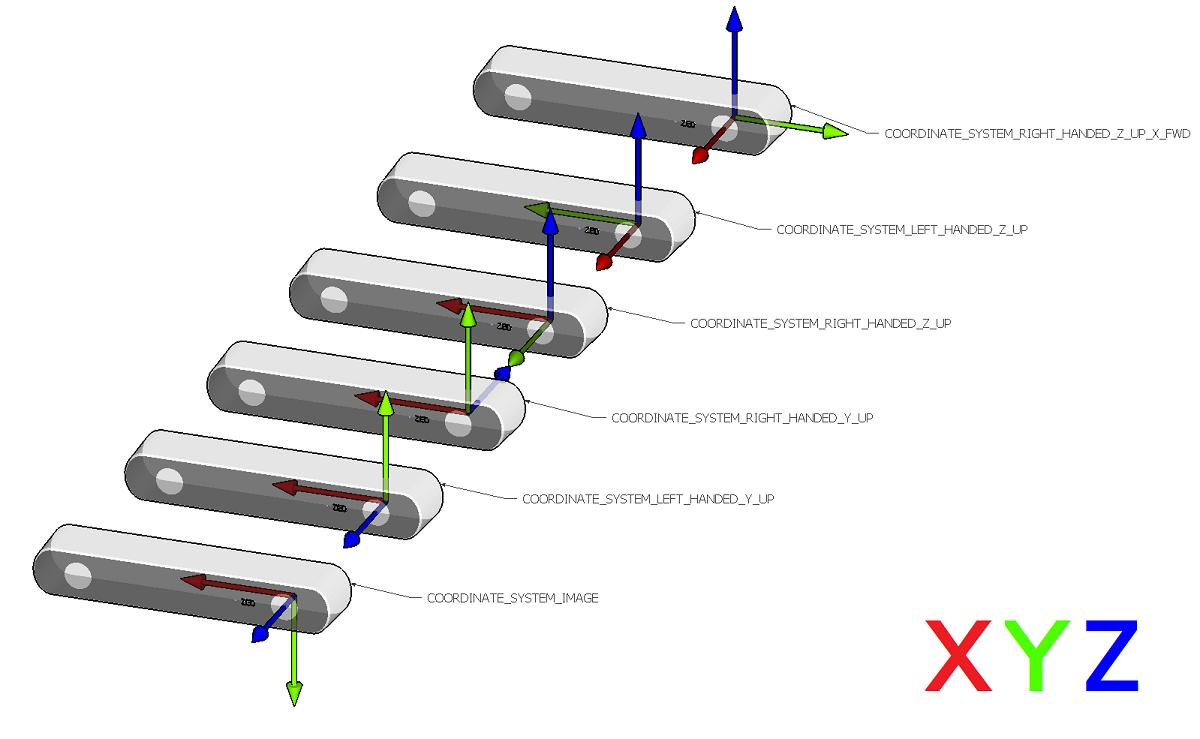
\includegraphics[height=6cm]{immagini/CoordinateSystem}
	\caption{Sistemi di rifermento messi a disposizione dalla nostra fotocamera stereoscopica.}
	\label{figura:sdrZED}
\end{figure}
\\\indent Di seguito, analizziamo la struttura del file relativo all'attività \texttt{ObjectDetection}. Le prime due funzioni dell'attività sono il costruttore e il distruttore della classe, mentre la terza funzione è la callback relativa alla connessione. La callback relativa alle informazioni delle fotocamera, invece, è organizzata nel seguente modo: 
\begin{itemize}
\item \textit{Acquisizione delle immagini dallo slot del CAB}: nella nostra applicazione serve solo la point cloud, che viene memorizzata in una struttura dati di tipo \texttt{cv::Mat};
\item \textit{Rilascio dello slot del CAB appena utilizzato}: in seguito al salvataggio della point cloud, possiamo rilasciare lo slot del CAB per renderlo nuovamente disponibile a contenere nuovi dati;
\item \textit{Impostazione delle soglie}: è \textbf{facoltativa}. Dal momento che questa libreria è sprovvista del classificatore, le soglie servono per individuare l'oggetto da afferrare in uno scenario complesso. A queste variabili, bisogna assegnargli il valore massimo e minimo, espresso in metri e rispetto al sistema di riferimento della telecamera, della regione di spazio in cui può trovarsi l'oggetto;
\item \textit{Conversione del formato dei dati della point cloud}: è un passaggio necessario, dal momento che i dati della telecamera sono memorizzati in una matrice \texttt{cv::Mat}, mentre la nostra libreria richiede in ingresso una struttura dati della libreria \textit{PCL} (\texttt{pcl::PointCloud<pcl::PointXYZRGBA>::Ptr}). Per effettuare questa conversione, copiamo il contenuto di ogni cella della prima variabile, che sono un insieme di quattro \texttt{double}, nel corrispondente campo della variabile di tipo \texttt{pcl::PointXYZ-}\\\texttt{RGBA}, quindi effettuiamo il \textit{push back} di quest'ultima variabile nella struttra dati della libreria \textit{PCL} di nostro interesse. Il punto in esame viene inserito solo se tutti i campi della cella di partenza non sono \texttt{NaN}, altrimenti non avrebbe significato;
\item \textit{Estrazione dei soli punti appartenenti all'oggetto}: è \textbf{facoltativa}. Quest'elaborazione serve solo in scenari complessi ed utilizza le soglie impostate in precedenza. Il vettore dei punti costruito al punto precedente viene scandito interamente, così che nella nuova struttura dati relativa alla point cloud siano contenuti solo i punti che costituiscono l'oggetto da afferare;
\item \textit{Conversione della point cloud ed estrazione dei soli punti appartenenti all'oggetto}: è \textbf{facoltativa}. In questa funzione vengono eseguiti simultaneamente gli ultimi due punti appena descritti, è stata creata solo per motivi di ottimizzazione temporale. Infatti, l'estrazione di determinati punti richiede di scandire completamente il vettore dei punti, e visto che questo è costituito all'incirca da 100.000 elementi, la scansione risulta essere troppo onerosa in termini di tempo, quindi si è scelto di creare anche una versione che svolge allo stesso tempo entrambe le elaborazioni. L'utente finale può utilizzare la versione che preferisce e commentare quella che non intende utilizzare;
\item \textit{Chiamata del plugin \texttt{arm\_grasp\_gcg}}: dopo che la point cloud è stata convertita nel formato richiesto ed elaborata come necessario per l'applicazione, può essere passata come parametro della funzione che richiama il plugin della libreria GPG. Il nome della variabile è determinato dall'elaborazione che si è scelta di utilizzare;
\item \textit{Salvataggio su log del vettore delle prese}: le prese ritornate dal plugin che richiama la libreria GPG vengono salvate sul log \texttt{ObjectDetection.log} nella cartella \texttt{bin}, in questo modo sono consultabili per analizzare i dati sulle prese ritornate dal plugin;
\item \textit{Creazione di un messaggio contenente il vettore delle prese}: le prese ritornate dal plugin vengono memorizzate in un messaggio di tipo \texttt{GraspCandidates} (la cui descrizione dettagliata si trova nella sezione \ref{messages}), successivamente il messaggio viene pubblicato. Questo passaggio è utile nel caso in cui le informazioni sulle prese servono ad altre attività o componenti. All'interno del ciclo \texttt{for}, è anche possibile specificare se accettare o meno una determinata presa, per esempio imponendo delle condizioni sull'orientamento. Per fare questo, si può ottenere l'orientamento secondo la notazione RPY grazie alla funzione \texttt{getRPY} della classe \texttt{Transform3D} e imporre i vincoli desiderati.
\end{itemize}
Ogni volta in cui si apportano delle modifiche ad un'attività, è necessario ricompilare il componente scrivendo \texttt{.~compile.sh} nel terminale. Invece, per eseguire il componente, bisogna scrivere \texttt{.~run.sh} nel terminale. In entrambi i casi, il comando va digitato all'interno della cartella \texttt{bin} del componente d'interesse.
\section{Messages}\label{messages}
Per quanto riguarda i messaggi, per la nostra applicazione è risultato necessario utilizzare i messaggi di tipo \texttt{manipulation\_msgs} disponibili nella cartella \texttt{Messages} di STAR e in particolare abbiamo dovuto introdurre nel file \texttt{manipulation\_msgs.idl} una nuova tipologia di struttura dati denominata \texttt{GraspCandidates}. Questa struttura consente di contenere al suo interno le possibili pinze individuate dalla libreria GPG ed è composta a sua volta da un campo corrispondente a una sequenza di oggetti di tipo \texttt{GraspPose}. Questa è un'ulteriore struttura dati che abbiamo creato in modo da rappresentare la singola pinza ed è costituita da tre campi di tipo \texttt{Transform3D}, che a sua volta è una nuova struttura dati introdotta che serve per rappresentare la traslazione e la rotazione della pinza. I tre campi della struttura \texttt{GraspPose} si distinguono in base al tipo di traslazione individuata:
\begin{itemize}
	\item \texttt{coord\_bottom}, contiene le coordinate della traslazione fra il sistema di riferimento della telecamera e la posizione centrata sulla base della pinza del robot;
	\item \texttt{coord\_top}, contiene le coordinate della traslazione fra il sistema di riferimento della telecamera e la posizione centrale fra le estremità delle dita della pinza del robot;
	\item \texttt{coord\_surface}, contiene le coordinate della traslazione fra il sistema di riferimento della telecamera e la posizione centrata sulla superficie dell'oggetto.
\end{itemize}
L'ultima struttura dati creata, \texttt{Transform3D}, è formata da 7 campi di tipo double, di cui i primi tre permettono di rappresentare le traslazioni (x, y e z, chiamati rispettivamente \texttt{a}, \texttt{b} e \texttt{c} per avere dei nomi univoci), mentre gli ultimi quattro rappresentano le rotazioni espresse sotto forma di quaternioni (\texttt{x}, \texttt{y}, \texttt{z} e \texttt{w}). \par
Una volta apportate le precedenti modifiche al file \texttt{manipulation\_msgs.idl}, è necessario ricompilare i messaggi tramite i seguenti comandi in un nuovo terminale: 
\begin{verbatim}
  cd STAR/AutonomousRobots/Messages
  . compile.sh
\end{verbatim}
La compilazione va eseguita tutte le volte che si modificano i messaggi.

\newpage
\chapter{Risultati}\label{risultati}
La libreria è stata testata inquadrando una bottiglietta posta ad una distanza di circa \SI{70}{c\meter} dalla fotocamera. Di seguito, si riportano la fotografia della scena inquadrata (figura \ref{figura:scenalab}) ed il grafico delle prese individuate (figura \ref{figura:preselab}). 
\begin{figure}[h!]
	\centering
	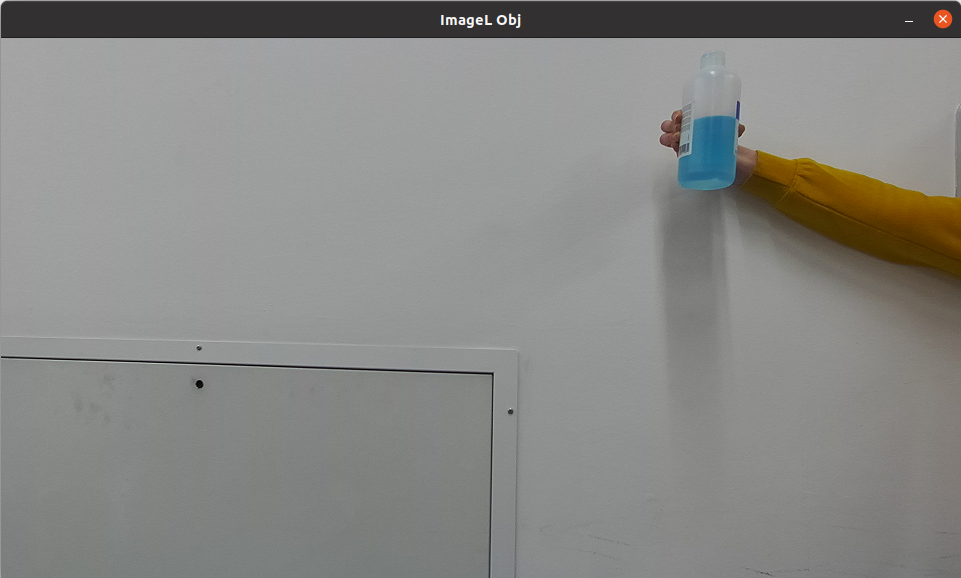
\includegraphics[height=6.9cm]{immagini/lab3}
	\caption{Scena inquadrata con la fotocamera stereoscopica.}
	\label{figura:scenalab}
\end{figure}
\begin{figure}[h!]
	\centering
	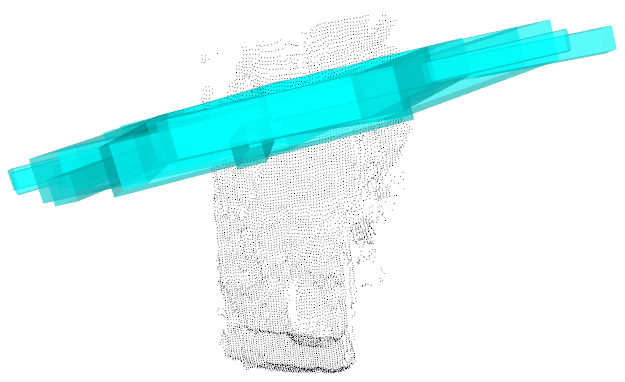
\includegraphics[height=5.5cm]{immagini/lab1}
	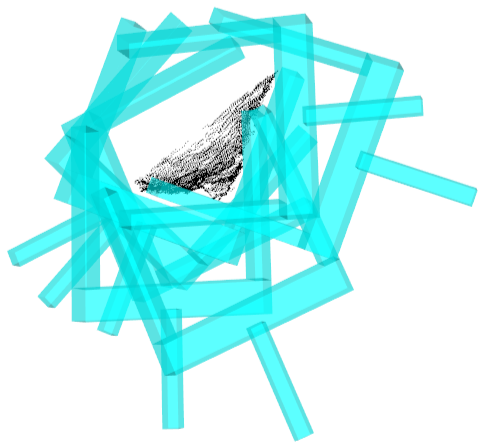
\includegraphics[height=5.5cm]{immagini/lab2}
	\caption{Point cloud con le prese vista frontalmente (a sinistra) e dall'alto (a destra).}
	\label{figura:preselab}
\end{figure}
\\Successivamente, le coordinate delle prese sono state utilizzate da un robot manipolatore a 6 gradi di libertà. In questo caso, nel file di configurazione del nostro componente è stato necessario cambiare il numero del dominio sul quale pubblichiamo il messaggio, per fare in modo che questo possa essere letto dal componente che gestisce il manipolatore. Inoltre, per semplicità di utilizzo, il nostro progetto è stato integrato in quello del manipolatore, così che si potessere gestire da un unico computer i due componenti. Di seguito, si riportano alcune fotografie dello scenario in cui è stata testato il nostro progetto.
\begin{figure}[h!]
	\centering
	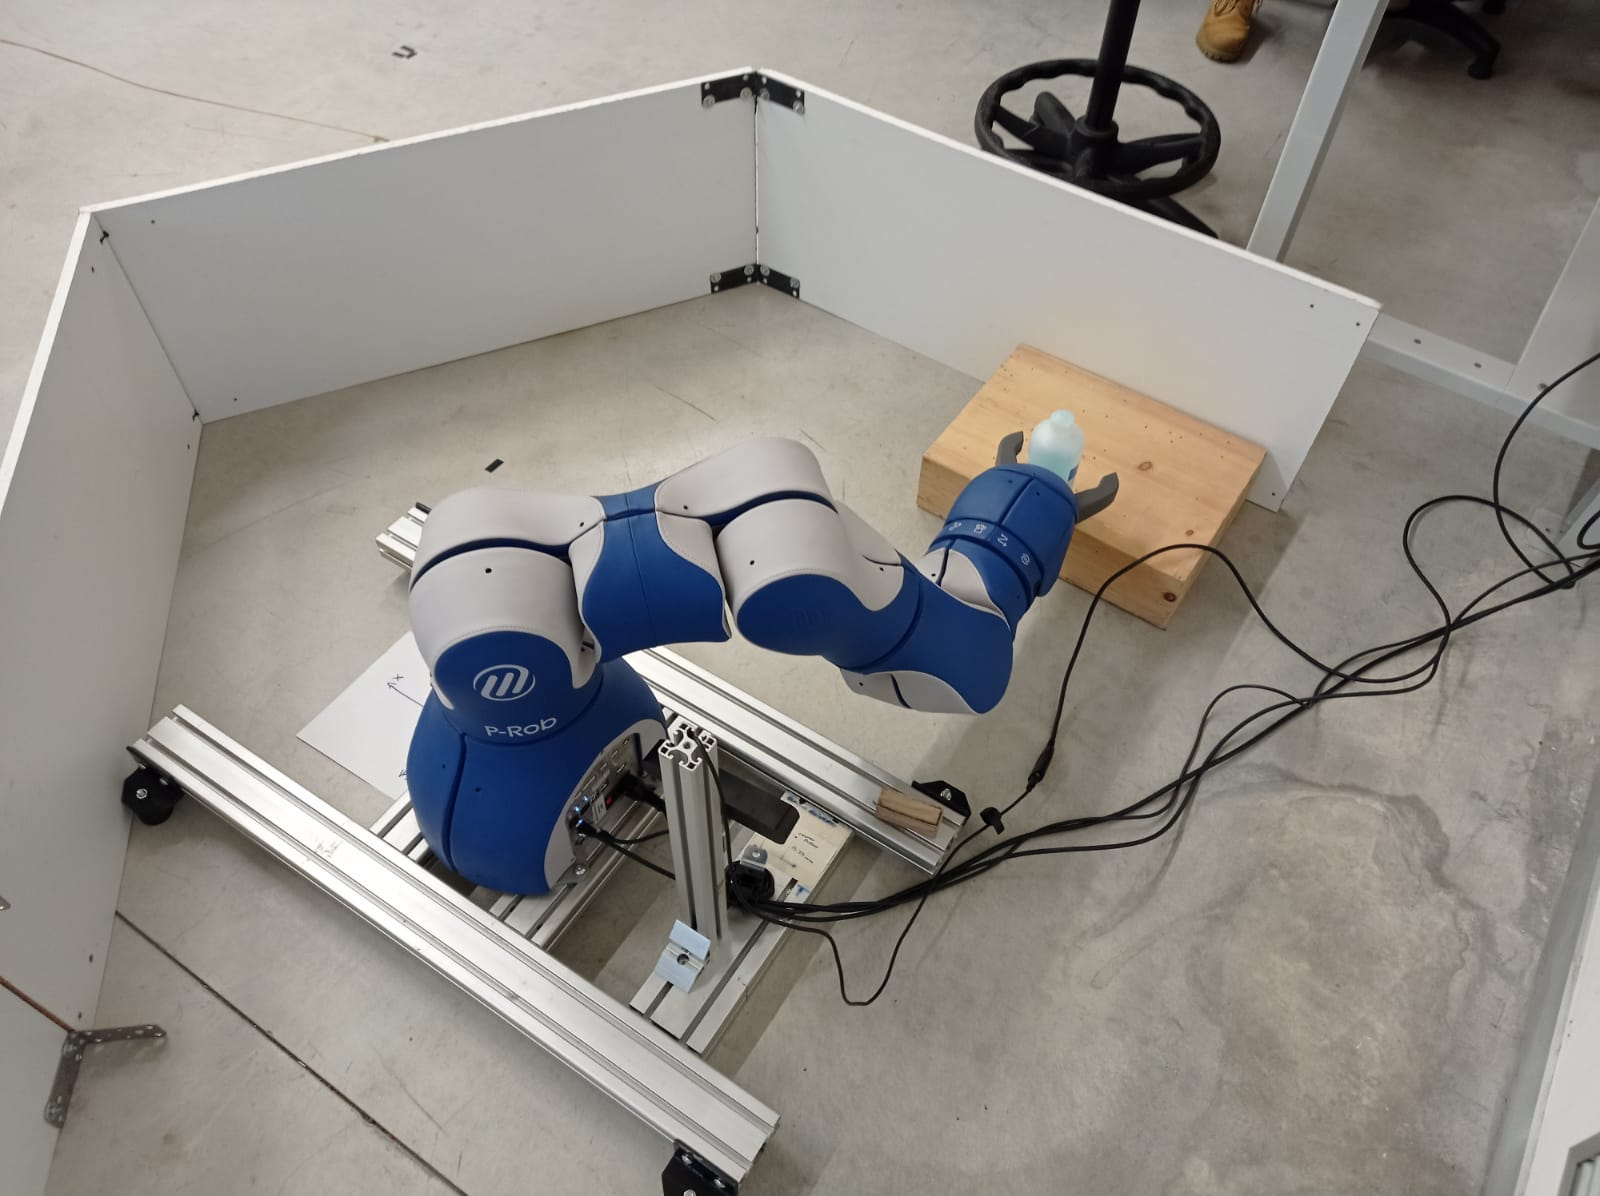
\includegraphics[width=\textwidth]{immagini/manipAlto}
	\caption{Fotografia della scena vista dall'alto.}
	\label{figura:manipAlto}
\end{figure}
\begin{figure}[h!]
	\centering
	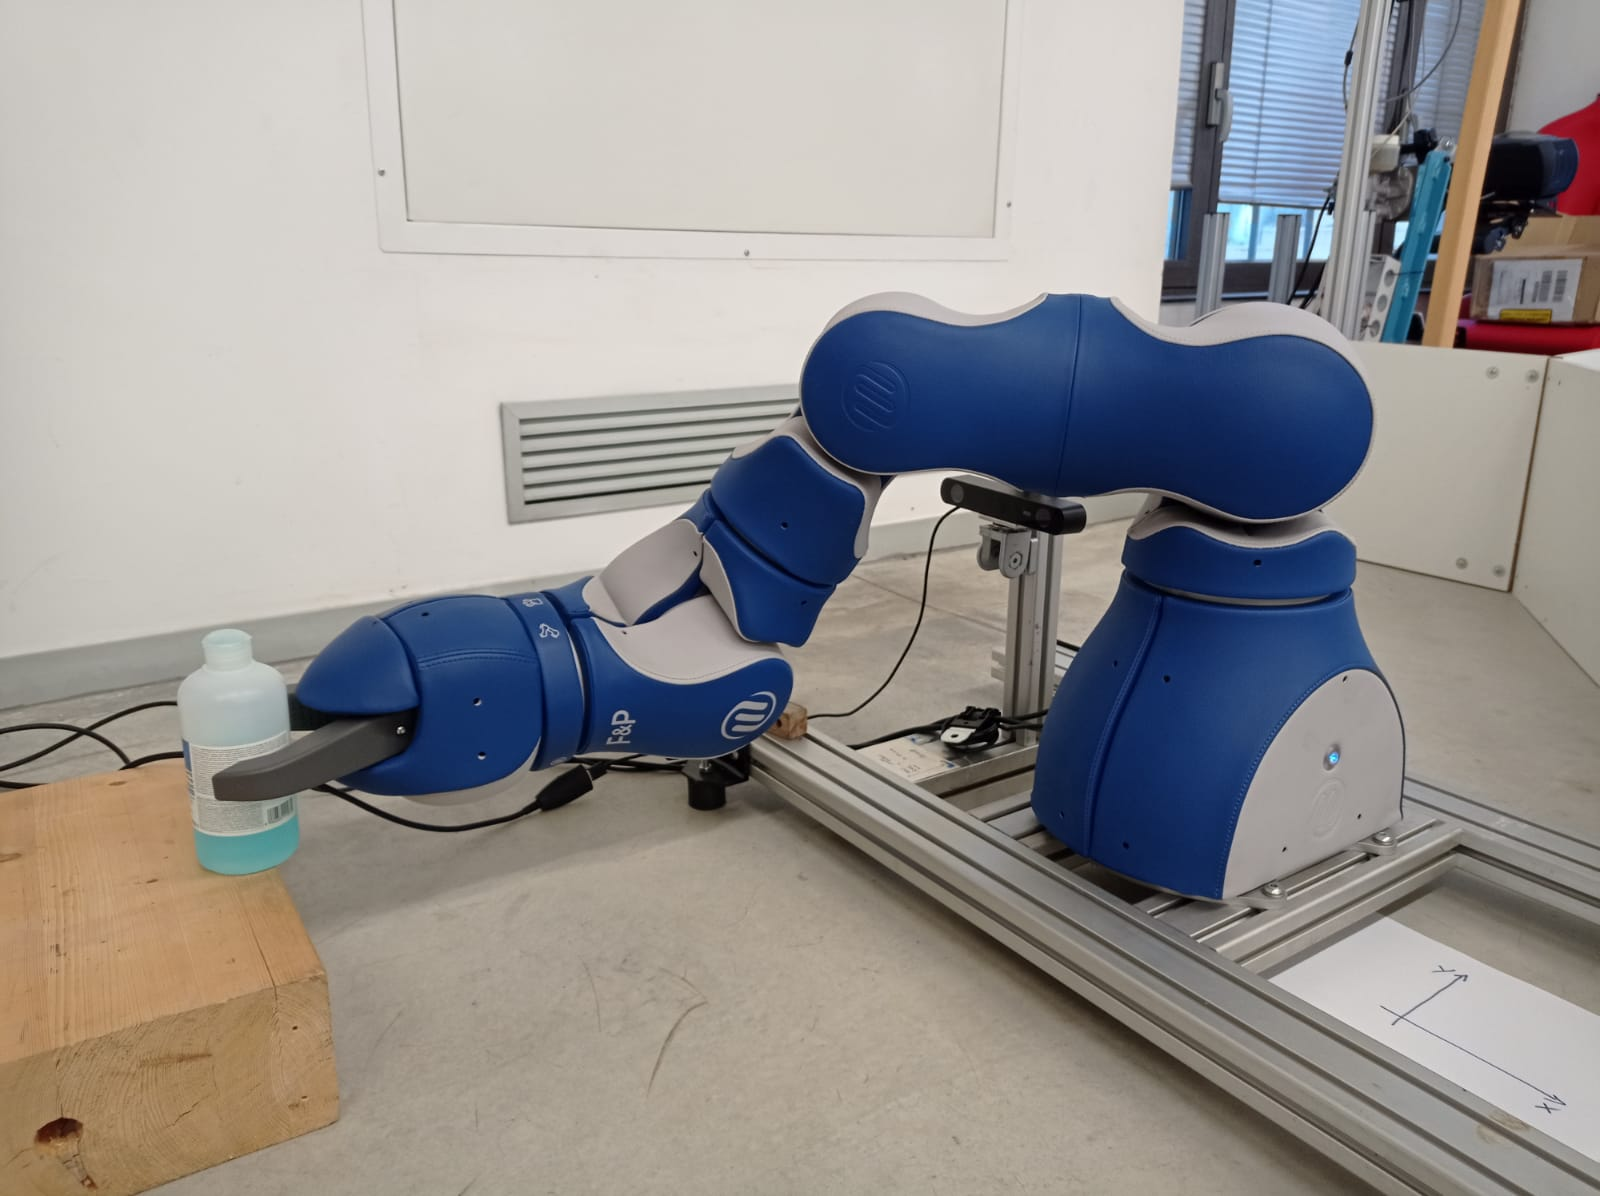
\includegraphics[width=\textwidth]{immagini/manipDavanti2}
	\caption{Fotografia della scena vista lateralmente.}
	\label{figura:manipDavanti}
\end{figure}
%----------------------------------------------------------------------------------------

\end{document}
